\documentclass{llncs}
%\usepackage{llncsdoc}
\usepackage{epsfig}
\usepackage{graphicx}

%\usepackage{caption}
%\usepackage{subcaption}

\newtheorem{mydef}{Def.}
\newtheorem{myhyp}{Hypothesis}

\usepackage{url}
\usepackage{hyperref}

\pagestyle{empty}

% PAKDD 2018: maximum 12 pages
% Abstract max 200 words
% title, abstract: 1/2 page
% introduction: 1 1/2 page (2 pages so far)
% related work: 1 to 1 1/2 pages (3 pages so far)
% method: 4 pages (7 pages so far)
% experiments: 3 (10 pages so far)
% discussion /conclusion: 1 page
% citations 1

% ====================================================================

% Eamonn ICDM'10 tutorial slides
% - clear problem statement in abstract
% - To convince a reviewer, you must think like a reviewer

% Writing the paper:
% - Make a working title
% - Introduce the topic and define (informally at this stage)
%   terminology
% - Motivation: Emphasize why is the topic important
% - Relate to current knowledge: what’s been done
% - Indicate the gap: what need’s to be done?
% - Formally pose research questions
% - Explain any necessary background material.
% - Introduce formal definitions.
% - Introduce your novel algorithm/representation/data structure etc.
% - Describe experimental set-up, explain what the experiments will
%   show
% - Describe the datasets
% - Summarize results with figures/tables
% - Discuss results
% - Explain conflicting results, unexpected findings and discrepancies
%   with other research
% - State limitations of the study
% - State importance of findings
% - Announce directions for further research
% - Acknowledgements
% - References
%
% - Don’t make the reviewer of your paper think!
% - Reviewers make an initial impression on the first page and don’t
%   change 80% of the time
% - A good introduction with a good motivation is half your success
% - By the end of the introduction the reviewer mustknow.
%   - What is the problem?
%   - Why is it interesting and important?
%   - Why is it hard?why do naive approaches fail?
%   - Why hasn't it been solved before?(Or, what's wrong with previous
%     proposed solutions?)
%   - What are the key components of my approach and results?Also
%     include any specific limitations.
%   - A final paragraph or subsection: “Summary of Contributions”.
%     It should list the major contributions in bullet form,
%     mentioning in which sections they can be found. This material
%     doubles as an outline of the rest of the paper, saving space and
%     eliminating redundancy
% - Unjustified Choices (are bad)
% - Optimal: Does not mean `very good'
% - Proved: Does not mean `demonstrated'
% - Significant: There is a danger of confusing the informal statement
%   and the statistical claim
% - Use all the Space Available
% - Avoid Weak Language: aim, attempt, might, etc.
% - Use the Active Voice
% - ALWAYS put some variance estimate on performance measures (do
%   everything 10 times and give me the variance of whatever you are
%   reporting)

% Figures:
% - Don't cover the data with the labels!
% - Color helps -Direct labeling helps -Meaningful captions help
%
% Common problem with figures:
% 1.Too many patterns on bars
% 2.Use of both different symbols and different lines
% 3.Too many shades of gray on bars
% 4.Lines too thin (or thick)
% 5.Use of three-dimensional bars for only two variables
% 6.Lettering too small and font difficult to read
% 7.Symbols too small or difficult to distinguish
% 8.Redundant title printed on graph
% 9.Use of gray symbols or lines
% 10.Key outside the graph
% 11.Unnecessary numbers in the axis
% 12.Multiple colors map to the same shade of gray
% 13.Unnecessary shading in background
% 14.Using bitmap graphics (instead of vector graphics)
% 15.General carelessness

% ====================================================================

% TODO:
% - clearly point out novelty of this work
% - contribution compared to earlier work

\begin{document}

% ====================================================================
% Previous title versions
\iffalse  

% Peter 31 Oct: Current title does not really reflect the topic I think:
%\title{Exploring approaches to probabilistic record linkage using similarity searching}
% Peter 31 Oct: What about
\title{Efficient and Effective Metric Space Indexing for Complete Record Linkage}
       
\fi
% ====================================================================
       
\title{Using Metric Space Indexing for Efficient Complete Record Linkage}

\author{Submitted for double-blind review}

% ====================================================================
%  Hidden For Blind Review
\iffalse  

\author{{\"O}zg{\"u}r Akg{\"u}n\inst{1} \and Alan Dearle\inst{1} \and Graham Kirby\inst{1}
\and Peter Christen\inst{2}}

\institute{School of Computer Science, University of St Andrews, St Andrews, Scotland.\\
Contact: \email{ozgur.akgun@st-andrews.ac.uk}
\and
Research School of Computer Science, The Australian National University, Canberra, Australia.\\
Contact: \email{peter.christen@anu.edu.au}}
      
\fi
% ====================================================================

\maketitle

\begin{abstract}
%Probabilistic
Record linkage is the process of identifying records that refer to the
same real-world entities, in situations where entity identifiers are
unavailable. Records are linked on the basis of similarity between
common attributes, with every pair of records being classified as a
match or non-match depending on the degree of similarity between them.
Record linkage is usually performed in a three-step process, where first
groups of similar candidate records are identified using indexing. Only
pairs within the same group are then compared in more detail, and
finally classified.
%
Even state-of-the-art indexing techniques, such as Locality Sensitive
Hashing, have potential drawbacks. They may fail to group together some
true matching records with high similarity. Conversely, they may group
records with low similarity, leading to high computational overhead.
%
We propose using metric space indexing to perform \emph{complete} record
linkage, which results in a parameterless record linkage process
combining indexing, comparison and classification into a single step
delivering high effectiveness and efficiency.

\end{abstract}

\keywords Entity resolution; data matching; similarity search;
         blocking.

% ====================================================================

% 1 1/2 pages maximum!

\section{Introduction}
\label{sec-intro}

% Peter, 20171112:

Record linkage, also known as entity resolution, data matching and
duplicate detection~\cite{Chr12}, is the process of identifying and
matching records that refer to the same real-world entities within or
across databases. The entities to be linked are often people (such as
patients in hospital or customers in business databases), but record
linkage can also be applied to link consumer products or bibliographic
records~\cite{Chr12}. Record linkage is commonly challenged by the lack
of unique entity identifiers (keys) in the databases to be linked, which
prevents the use of a database join. Instead, the linkage of records
requires the comparison of the common attributes (or fields) that are available
in the datasets to be linked. For datasets that contain
information about individuals, these attributes include the names,
address, dates of birth, and so on, of individuals.

To overcome data quality issues such as typographical errors and
variations (which are common in name and address values~\cite{Chr12}),
approximate string comparison functions (such as edit distance, the
Jaro-Winkler comparator, or Jaccard similarity~\cite{Chr12}) are used to
compare pairs of records, leading to a vector of similarities (one
similarity per attribute/field compared) for each pair. These similarity
vectors are then used to classify the compared record pairs into matches
(where it is assumed both records in a pair correspond to the same
real-world entity) and non-matches (where the records are assumed to
correspond to two different entities). Various classification methods
have been employed in record linkage~\cite{Chr12,Don15}, ranging from
simple threshold based to sophisticated clustering, supervised
classification techniques, and active learning approaches~\cite{Wan15}.

Besides the issues of a lack of unique entity identifiers, and data
quality (which will affect linkage quality), record linkage is also
challenged by the increasing sizes of the datasets to be
linked~\cite{Don15}. To avoid full pair-wise comparison of all possible
record pairs (quadratic in the sizes of the datasets to be linked),
blocking techniques, commonly known as \emph{indexing}~\cite{Chr12b},
are used. These split the datasets into smaller blocks in a
computationally efficient way, such that records that are likely to
correspond to the same entity are grouped into the same block. Only
records within the same block are then compared in more detail.

While indexing techniques facilitate efficient linkage of very large
datasets~\cite{Don15}, they generally achieve scalability at the cost
of reduced linkage quality, because potentially true matching record
pairs are removed in the indexing step, leading to a reduction in recall
of the final linkage result~\cite{Chr12}. A variety of indexing
techniques, discussed in more detail in the following section, have
been proposed, ranging from simple phonetic based blocking~\cite{Chr12}
and sorting of the datasets~\cite{Dra12} to locality sensitive hashing
based techniques~\cite{Kim10,Steorts2014}. Techniques for
unsupervised~\cite{Kej13,Ram15} and supervised~\cite{Bil06,Mic06}
learning of optimal blocking schemes have also been proposed.

\begin{figure}[!t]
  \centering
  %\scalebox{1.0}[1.0]
  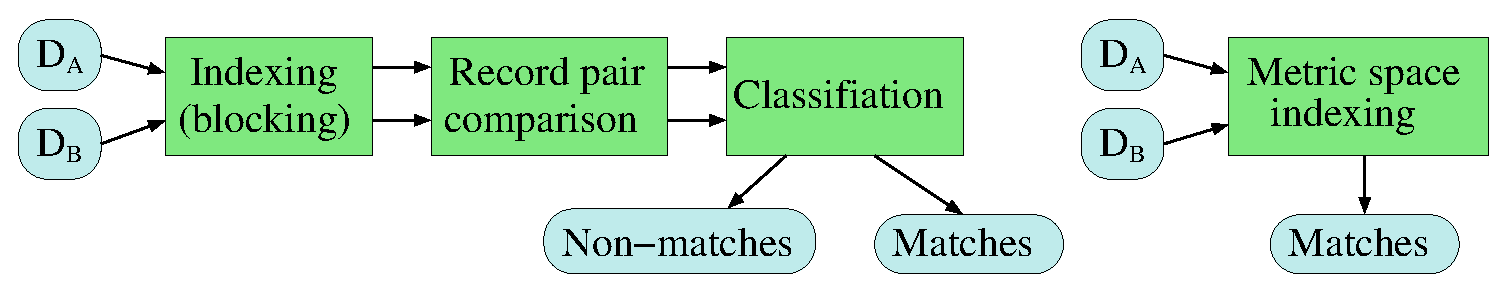
\includegraphics[width=1.0\textwidth]{figures/linkage-process}
  \caption{Overview of the steps of the traditional record linkage
           process (left-hand side) and our proposed metric space
           indexing based approach (right-hand side), as described in
           Sect.~\ref{sec-intro}, where records from two databases,
           $\mathbf{D}_A$ and $\mathbf{D}_B$, are being linked.}
           \label{fig-rl-process}
\end{figure}

Systems that perform indexing prior to comparison and classification, as
illustrated in Fig.~\ref{fig-rl-process}, add a further practical
complexity to the process. Indexing, comparison and classification are
often conducted using algorithms and parameters selected based on
technical and domain expertise of the user of the record linkage system,
followed by a manual assessment (auditing) of the linkage
outcomes~\cite{Chr12}. If the quality of the resulting links is not good
enough for a certain application, the linkage process needs to be
repeated with different parameter settings and possibly also alternative
algorithms. This can result in a time-consuming and labor-intensive
iterative process. A major challenge is often the heuristic nature of
indexing, where the choice of a certain indexing technique and its
parameters (including which attributes to use in indexing) will
determine the final outcome of a linkage.

% Repeat:
% If a certain blocking approach results in a loss of recall in the
% final linkage results, as determined by post auditing, the blocking
% needs to be redone, an often time consuming process.

Here we explore how existing indexing techniques can lead to
reduced recall, even for record pairs that are highly similar and likely
correspond to true matches. As a result, such techniques can lead
to \emph{incomplete} record linkage results. To address this problem,
\emph{metric space indexing} (MSI) can be used to guarantee that all
record pairs, up to a certain distance threshold, are considered in the
record linkage results. MSI also avoids the need for costly detailed
comparison of record pairs with low similarities, which may be inserted
into the same block with traditional indexing techniques. It allows
indexing, comparison and classification to be combined into a
single step, as shown in Fig.~\ref{fig-rl-process}, making the overall
record linkage process simpler, more efficient and more effective than
the traditional approach.

% Sanity check this claim in final version.

% Peter 20171112: do we also need to mention we do not waste
% comparisons of record pairs with low similarities (i.e. those with
% a distance > max_dist)?


%to add: something about similarity spaces / metric spaces, M-trees and its more recent advanced/improved versions, and how they have been used in similarity search.}
%to add: How our work is different from these other metric space works, and description of our contributions.

\smallskip
%Al - I have beefed this up and added a fourth contribution.
\textbf{Contributions:} We make four specific contributions: (1) We
investigate how existing indexing techniques can result in
\emph{incomplete} record linkage results. (2) We show that these
techniques are highly sensitive to parameter settings and can produce
very low quality linkage. (3) We explore MSI for record linkage and
propose an approach that achieves consistently \emph{complete},
efficient and effective record linkage. (4) We evaluate our approach on
several data sets from diverse domains and show its advantages over
existing indexing techniques for record linkage.

% TODO: check that the above claims have been addressed.

% *******************************************************
% we can't write this as it reveals us in the double-blind review
% we can add to final paper:
% The motivation for this work is the Digitising Scotland project (Dibben 2012), which is in the process of transcribing and linking all the vital events recorded in Scotland between 1856 and 1977. This data set will, when complete, include around 14 million birth records, 11 million death records and 4 million marriage records. As part of the work, certain data fields (locations, occupations and causes of death) are also being classified to the relevant standard coding schemes.
% *********************************************************

% --------------------------------------------------------------------

\section{Related Work}
\label{sec-related}

We now briefly review relevant work in the areas of indexing
for record linkage (for recent surveys see~\cite{Chr12b,Pap16}),
and metric space indexing~\cite{Zezula2010}.

\smallskip
\textbf{Indexing for Record Linkage:}
Techniques to link records across datasets have been investigated for
over five decades~\cite{Fel69,New59} with the scalability of linking
being an ongoing challenge as datasets continue to grow in size and
complexity. Traditional blocking~\cite{Chr12b} uses a set of attributes
(known as a \emph{blocking key}) to insert records that share the same
value(s) in their blocking key into the same block. Only records within
the same block are  compared to each other. To overcome variations and
misspellings, the values used in blocking keys can be phonetically
encoded using functions such as Soundex, NYSIIS, or
Double-Metaphone~\cite{Chr12}. These techniques convert a string  into a
code according to its pronunciation, assigning the same code to similar
sounding names (such as `Gail' and `Gayle').

A different approach to indexing is the sorted neighborhood
method~\cite{Mon96}, where the datasets to be linked are sorted
according to a \emph{sorting key} (usually a concatenation of the values
from several attributes). A sliding window is then moved over the
datasets and only records within the window are compared. Techniques
that adaptively shrink or expand the window size based on the
characteristics of the sorting key values have shown to improve both
linkage efficiency and quality~\cite{Dra12} over other sliding window
approaches.

These blocking techniques are heuristics, commonly requiring domain
knowledge, such as the choice of appropriate blocking or sorting keys.
Poor choices of blocking attributes result in records being inserted
into a wrong block and thus true matches being missed. As a result,
existing blocking techniques can lead to \emph{incomplete} linkage.
Conversely, many of the record pairs compared in a block turn out to be
pairs with low similarities, corresponding to non-matches, resulting in
\emph{inefficient} linkage.

Locality sensitive hashing (LSH), originally proposed to allow
efficient nearest-neighbor search in high-dimensional
spaces~\cite{Ind98}, has been employed in record linkage as a blocking
technique where attribute values are hashed multiple times, and
blocks are created from those records that share some hash values.
\emph{HARRA} is a record linkage approach based on Min-hash and LSH
which blocks, compares, and then merges linked records in an iterative
fashion, where merged records are re-hashed to improve overall linkage
quality. Steorts et al.~\cite{Steorts2014} recently evaluated two LSH
variations, with their main conclusion being that in order to get good
results LSH methods must be tuned to the particular datasets being
linked. This requires good quality ground truth data which may be
unavailable or very expensive to obtain.

Metric space indexing (MSI) techniques require indexing structures to be constructed over a set of records that are then used to support comparison with another set. MSI data structures often support a rich set of similarity search operations over a set of values over a metric space (distances must support the triangle inequality). The operations supported include \textit{range search} where all objects $i$ within a distance $d$ for a query object $q$ are identified, i.e.\ $dist(i,q) \le d$) \textit{nearest-neighbour} (the closest value to q), and \textit{nearestN} (the N closest n objects to q). An overview of the many Metric space search techniques that are available may be found in \cite{Zezula2010}. In this paper we choose one metric space data structure the M-Tree \cite{paolociaccia2m} and investigate its efficacy for record linkage.

An M-tree is a balanced tree structure comprised of fixed sized nodes each have a fixed number of children. In addition to the children, each node contains a reference to an object being indexed, a pointer and the distance to its parent, and a radius (described below). The radius of an internal node called a \textit{routing-node} represents the  furthest distance to any of its children. Thus all the children may be visualised as being contained within a ball of radius \textit{r} from the parent. M-trees are grown from the roots upward and require dynamic tree rebalancing when set of children become full (of size \textit{M}).

Yu et al. \cite{Yu2016} have written an extensive survey on the use of string similarity and join for record linkage and define the problem as "Given two sets of objects, similarity join aims to find all similar pairs from the two collections". Part of the survey is concerned the algorithms used to compare two records which are characterised as being character-based, token-based or hybrid. The first, which includes approaches such as Levenshtein~\cite{Levenshtein66}, use character differences in the strings being compared, the second, which includes techniques such as Jaccard similarity, which treat the records as sets of tokens and utilises set similarity, the third hybridises the two approaches. Yu's divides join algorithms (which unify records - also known as linkage) into three categories: a number of techniques based on filtering, verification based and threshold-based. Filtering involves generating signatures for each record and creating inverted lists containing records with common signatures and pruning records with no common signatures. Verification algorithms involve calculating the exact distances of a prefix of the data, and using another technique to estimate the edit distance between records. If the estimated distance is larger than the desired similarity threshold, the candidate may be discarded. The last category (threshold based) includes M-trees, Trie-Join, Pass-Join and Partenum.  

\cite{Li2006} describes a method of performing linkage using R-trees~\cite{Hjaltason1998} that fall into the threshold based category of Yu et al. Their approach demonstrated that high precision and recall may be achieved by measuring Jaccard similarity over selected fields from set of records being compared. In their evaluation, their approach achieved a recall of 99 percent in experiments in which conjunctions of similarities over fields were used. In a later paper \cite{Ciaccia97indexingmetric}  Ciaccia et al. demonstrate that using M-trees are almost always more efficient than R-trees and hence their use in the experiments described in this paper.

% end of related work should be around end of page 3!

% --------------------------------------------------------------------

% do we need a section on preliminaries, notation, etc?
% ideally techniques are described formally, possibly via pseudo-code
% algorithmic descriptions

\section{Approach}
\label{sec-approach}

% peter: We need one paragraph describing the overall 'approach' /
% methodology, as well as the aim, then a short description of
% each method/technique used

% would be good to have a figure if possible illustrating these
% approaches

% Graham - should it be complete/incomplete rather than exact/inexact below?
We explore the efficacy of several similarity search algorithms in
record linkage: one popular inexact algorithm, LSH-minhash, and one exact
method, M-tree~\cite{paolociaccia2m}. We also use a simple brute force
(nested-loop) exact technique as a baseline for comparison, although
this approach can only feasibly be applied to the smallest of our
datasets. All experiments have a number of parameters with which we can
configure the search space and algorithm behaviour, as described in
Sect.~\ref{sec-exp}. A \emph{distance threshold}, $d$, specifies a
maximum distance, equivalent to a minimum similarity, for two records to
be classified as a link (i.e.\ referring to the same entity).

\smallskip
\textbf{Nested loop:}
In the brute force approach two nested loops are used to compare every 
record with every other record. The complexity of this 
approach is quadratic in the number of records to
be linked. This approach is guaranteed to identify all links, i.e. record pairs within the given distance threshold, $d$.

% Needed? Apart from anything else, haven't introduced the datasets yet.
% Each of our datasets contains ground truth with which we can establish the records that are true links and those that are not. Clearly this approach can only be applied to relatively small datasets and we restrict its usage to the Cora dataset as a baseline for the other experiments.

\smallskip
\textbf{LSH-MinHash:}
The LSH-minhash algorithm used has three tuning parameters:
\emph{shingle size}, $l_{ss}$, the \emph{band size}, $l_{bs}$, and the
\emph{number of bands}, $l_{nb}$.
These are explained in the following algorithm description which follows a standard LSH approach [CITATION].
Using this approach, each record drawn from a set of records is placed in a \emph{LSH-MinHash} data structure.
To do this, for each record, firstly all the fields of the record are turned into strings and 
concatenated. Next the strings are \emph{shingled} into a set of
n-grams (sub-strings of length $n$) according to the $l_{ss}$
parameter (i.e.\ $n = l_{ss}$). Next a set of randomly, 
deterministically generated hash functions are applied to each of the
sets of n-grams and the smallest (the minhash) of each application is
added to a signature. The number of hashes used and thus the size of
the signature is set to $l_{nb} \times l_{bs}$.
Lastly the signature is divided into $l_{nb}$ segments and the elements from the band are hashed again to create a number of keys.
The original record is added to a hashmap associated with each of the keys. 
We we will evaluate the performance of LSH based blocking with regard to the three parameters $l_{ss}$, $l_{bs}$ and $l_{nb}$ in
Sect.~\ref{sec-exp}.
To perform linkage the following procedure is followed: for each query value is hashed using the procedure described above and the union of set of of values found for all hashes in the hashmap are returned. These are then be filtered by performing distance calculations on the results to eliminate false positives.

\smallskip 
\textbf{M-Tree:} The M-tree experiments have no parameters. In a similar manner to the \emph{LSH-MinHash} approach, M-trees are constructed by supplying the implementation with a set of records and a \emph{distance function}. The distance functions used are the same as those used for \emph{Nested-loop} and \emph{LSH-MinHash} experiments. To perform linkage the data-structure is searched using a \emph{range-search} query which yield all records within distance $d$ of the query object and all the returned records are directly recorded as links.


% - - - - - - - - - - - - - - - - - - - - - - - - - - - - - - - - - -

% subsection

%  - - - - - - - - - - - - - - - - - - - - - - - - - - - - - - - - - -

%\subsection

% --------------------------------------------------------------------

%  - - - - - - - - - - - - - - - - - - - - - - - - - - - - - - - - - -

%\subsection{Analysis and Limitations}
%\label{sec-analysis}

%maybe a complexity analysis? maybe an analysis of expected 
%linkage quality?

% --------------------------------------------------------------------

\section{Experiments and Results}
\label{sec-exp}

We now describe the data sets we use in our evaluation, the setup we
employed to evaluate our proposed metric indexing approach and
compare it with traditional blocking techniques, and we then present
and discuss our results.

% - - - - - - - - - - - - - - - - - - - - - - - - - - - - - - - - - -

% Peter 31 Oct: table style follows LNCS style guide

\begin{table}[t]
\caption{Characteristics of data sets used in the experiments.}
 \label{table-datasets}
  \centering
  \begin{scriptsize}
  %\addtolength{\tabcolsep}{-0.5pt}
  \begin{tabular}{cccc}
  \hline\noalign{\smallskip}
  Data set~ & ~Number of~ & ~Number of true~ & Attributes used \\
  name(s)  & records  & matching pairs & for traditional blocking \\
  \noalign{\smallskip} \hline \noalign{\smallskip}
  CORA  & 1,295 & 17,184 & Title, authors, venue, year ? \\
  NCVR  & ~224,073 / 224,061~ & ~148,036~ & ? \\
  Isle of Skye & 32,567 & 2,900 & ? \\
  Kilmarnock  & 70852 & 8,300 & ? \\
  \noalign{\smallskip} \hline
  \end{tabular}
  \end{scriptsize}
\end{table}

\smallskip
\textbf{Data Sets:}
%\label{sec-data}
We used four real data sets from three domains in our experiments as
summarized in Table~\ref{table-datasets}. The first is
\emph{CORA}~\footnote{Available from:
\texttt{http://secondstring.sourceforge.net}}, which contains 1,295
records that refer to 112 machine learning publications. Ground truth is provided via a unique
\emph{paper\_id} identifier of the form "blum1993".

The second are two snapshots of the North Carolina Voter Registration
database (\emph{NCVR})~\footnote{Available from: \texttt{http://dl.ncsbe.gov/}}, which were collected in April and June
2014. Each of these contains records of voters and includes their
first names, surnames, and addresses. Ground truth is provided via a
\emph{NCID} identifier which uniquely identifies a voter. In our
experiments we use two randomly selected sub-sets of $224,073$ and
$224,061$ records, respectively, where $148,036$ of those refer to
voters that occurred in both original NCVR snapshots but had name
and/or address changes over time (thus leading to around $66\%$
matching records).

The last two data sets are historical Scottish records of vital
events (birth, marriages and deaths) registered on the
\emph{Isle of Skye}, a rural district, while the other contains
records from \emph{Kilmarnock}, an industrial town. These data sets
were provided to us by the demographer and historians who extensively
curated and linked both data sets~\cite{reid2002,reid2006}. Both data
sets include the  names, gender, addresses of individuals and their
parents. Ground truth was generated by the demographers based on their
extensive domain knowledge.

% - - - - - - - - - - - - - - - - - - - - - - - - - - - - - - - - - - -

\begin{table}[t]
\caption{Parameter settings used for the different data sets used in
   the experiments,with $d$ the distance threshold used, $t_b$ the
   M-tree branching factor, $l_{ss}$, $l_{sb}$ and $l_{nb}$ the LSH
   shingle size, and the size and number of bands, respectively.
 \label{table-parameters}
  \centering
  \begin{scriptsize}
  %\addtolength{\tabcolsep}{-0.5pt}
  \begin{tabular}{cccccccc}
  \hline\noalign{\smallskip}
  Data set~ & $d$ & $t_b$ & $l_{ss}$ & $l_{bs}$ & $l_{nb}$ & 
    $f_{ki}$ & $f_{ks}$ \\
  name(s) & & & & & & & \\
  \noalign{\smallskip} \hline \noalign{\smallskip}
  CORA & ~$[0,5,10,\ldots,95,100]$~ & ~$[5,10,25,50]$~ & ~$2$~ &
    ~$[2,5,10]$~ & ~$[2,5,10]$~ & ~$[30,35,40]$~ & ~$[30,35,40]$ \\
  NCVR  &  \\
  Isle of Skye &  \\
  Kilmarnock  &  \\
  \noalign{\smallskip} \hline
  \end{tabular}
  \end{scriptsize}
\end{table}

\smallskip
\textbf{Experimental Setup:}
%
We implemented all techniques described in Sect.~\ref{sec-approach}
using Java (version 1.8.0\_144) and ran an extensive et of experiments on
a compute server with 24 Intel(R) Xeon(R) CPU E5-2630 processors running at 2.30GHz, 
128 GBytes of main memory and running Red Hat 4.8.5-11.

The parameter settings used in our experiments are summarized in
Table~\ref{table-parameters}. ... \emph{describe and justify selected
values..}

discuss measures used. PC, PQ, num comparisons, time? etc.

\subsection{Cora}

Do BruteForce, LSH and M-Tree

1.1 BruteForce



% - - - - - - - - - - - - - - - - - - - - - - - - - - - - - - - - - - -

\smallskip
\textbf{Results and Discussion}

%\subsection{Results and Discussion}
%\label{sec-results}

table or plots?

% --------------------------------------------------------------------

\section{Conclusions and Future Work}
\label{sec-concl}

% --------------------------------------------------------------------

\bibliographystyle{splncs03}
%\bibliographystyle{abbrv}
\bibliography{paper.bib} 

% ====================================================================

\end{document}

% ====================================================================

OLD STUFF

\section{The Plan}

\vspace{5mm}

Plan in a bulleted list:

\begin{itemize}
\item Design: Traditionally it has two stages. A blocking method needs to be developed separately from a similarity method. With similarity search based record linkage, there is only one method, and that is the similarity method.
\item Efficiency: I am not convinced of this, but Peter thinks there may be efficiency benefits. The reasoning behind this is that with blocking-based methods we would have to calculate some sort of a similarity value first. This value will only be used for blocking, and later a similarity value between candidate pairs will need to be calculated again.
\item Completeness: Similarity search based methods will be complete (with respect to the given similarity method) whereas blocking based methods (including LSH) are likely to be incomplete (there will be high-similarity pairs which are not places in the same block)
\item Data sets
\begin{itemize}
\item Kilmarnock Birth-Death
\item Skye Birth-Death
\item CORA
\item North Carolina Voter Registration DB
\end{itemize}
\item The following is a list of all methods we thought we would have to compare.
\begin{itemize}
\item Similarity search (M-Tree, others?)
\item LSH-blocking
\item Traditional blocking (e.g. Region, Surname) - \textbf{why this? - this was done in the paper: A Comparison of Blocking Methods for Record Linkage}
\item Sorted Neighbourhood blocking - \textbf{why this?}
\end{itemize}
\item Pairs-completeness and pairs-quality (w.r.t high similarity instead of true-link status). I will expand on this a bit more later.
\item Comparison (for blocking based methods)
		Precision/Recall/F1-Measure
\item Which similarity methods are metric?
\item Run time and memory usage comparisons
\item Theorem. Precision might get better or worse with similarity search based methods, but recall should never get worse.
\end{itemize}

Note: The rest of this paper should be regarded as a placeholder for now.

% ====================================================================

\smallskip
\textbf{MIfile:}
The MIFile \cite{amato2014mi} approach is an inexact technique for performing similarity search based on metric spaces. Using  MI\_file,  each record is represented by the ordering of distances from a collection of reference objects.
% Peter: are these reference object also records? 
It is based on the idea that two records close to each other will have similar neighbours and will thus be represented by similar of distances
% Peter: unclear what you mean with: similar of distances
from the chosen reference objects. 
In order to create the indexes, for each value to be added to the
% peter: value -> record ?
data-structure, first the k nearest reference objects (governed by a fixed parameter) are found, each is given a score (drawn from 1,2,3... based on the reference object's position from the value).
% peter: this is unclear .. I think I understand k-NN: for each
% record you find the k nearest reference objects and you enumerate
% them
Next for each score, a  mapping is created in an inverted index mapping
% peter: unclear..? a mapping in an inverted index mapping?
from the value to the score of each reference object and a representation of the data associated with the reference object and the value inserted.
% peter: unclear: what is "the data" associated with the reference
% object.
In order to perform a \textit{nearest-neighbour} lookup, first the k nearest reference objects (bounded by a second fixed parameter).
% peter: this sentence reads incomplete..?
Next the objects closest to these reference objects are extracted from the inverted map by choosing the neighbours with the highest score.
% Peter: sorry, this is unclear as well. "the objects closest" ->
% records closest? And why highest scores..? Is the closest record
% to a reference object given the highest score (not the lowest
% score - i.e. not 1-closest, 2-closest etc)
Much of the search space may be eliminated by  keeping track of the scores that  can contribute to the nearest neighbours.
% peter: so I guess you use the triangular inequality and the reference
% objects to prune the search space.


\if